\subsection{Convertidor CC-CC Conmutado}

Un convertidor CC-CC es un dispositivo electrónico que tiene como objetivo convertir una tensión continua, generalmente no regulada (es decir que no es fija), $V_{in}$ a la entrada, a una tensión continua regulada $V_{out}$ de distinta magnitud a la salida, transfiriendo la mayor cantidad de energía posible de la entrada hacia la salida. Dependiendo del tipo de convertidor, esta tensión de salida puede ser menor, mayor o tanto menor como mayor a la tensión de entrada.\\

Estos convertidores son de interés para nuestra aplicación, ya que la tensión $V_{stack}$ que entrega la pila (ecuación \ref{v_stack}) es una tensión continua no regulada, que varía apreciablemente con la corriente demandada; mientras que a la salida se demanda una tensión fija y regulada $V_{bus}$ para conectar al bus de continua del sistema híbrido de la figura \ref{SHGE}.\\

La forma más básica que se podría concebir para un dispositivo que cumpla esta función es la de un simple divisor resistivo, en el cual la tensión $V_{out}$ depende de las resistencias $R_1$ y $R_2$ y la tensión de entrada $V_{in}$.

\begin{equation*}
    V_{out} = V_{in}\cdot\frac{R_2}{R_1+R_2}
\end{equation*}

Entonces, variando la relación entre $R_1$ y $R_2$, se puede variar la tensión $V_{out}$ entre tensión nula y $V_{in}$. Sin embargo, se necesita solo un análisis superficial de esta topología para ver que no es viable, en especial para aplicaciones de alta potencia, más que nada por su pobre eficiencia energética (para obtener una tensión igual a la mitad de la entrada, se pierde la mitad de la potencia en disipación resistiva).\\

Los convertidores CC-CC se suelen separar en dos principales categorías: los {\Medium reguladores lineales}, que son un caso complejizado del divisor resistivo donde se utiliza un transistor como resistencia variable (además de un diodo para regular la tensión de salida); y los {\Medium convertidores conmutados}, en los cuales uno o más transistores, actuando como llaves, son conmutados a alta frecuencia y junto con dispositivos que almacenan energía (como inductores y capacitores) producen una tensión continua a la salida.\\

Dado que para esta plataforma se utiliza un convertidor conmutado (principalmente por su gran ventaja en eficiencia energética), se enfocará el análisis únicamente en éstos; comenzando por una explicación de los conceptos básicos necesarios para comprender su funcionamiento.\\

\subsubsection{Conceptos Básicos}

Como se detalló más arriba, los convertidores CC-CC conmutados consisten, en su forma más básica, en una fuente de continua no regulada a la entrada; y un transistor (que puede ser BJT, MOSFET o IGBT) que, mediante una excitación en su tercer terminal, se conmuta entre los modos de alta impedancia e impedancia nula, actuando como llave abierta y llave cerrada respectivamente. La proporción del tiempo total de ciclo ($T_s$) en la que el transistor está conduciendo ($t_{on}$) se denomina {\Medium ciclo de trabajo} o {\Medium \textit{duty cycle}} y se suele simbolizar con la {\Medium letra \textit{D}}. Como se verá más adelante, este es un parámetro crucial para el funcionamiento de este tipo de convertidores, ya que controlándolo se puede variar el nivel de tensión y corriente de salida.\\

\begin{figure}[h]
    \centering
    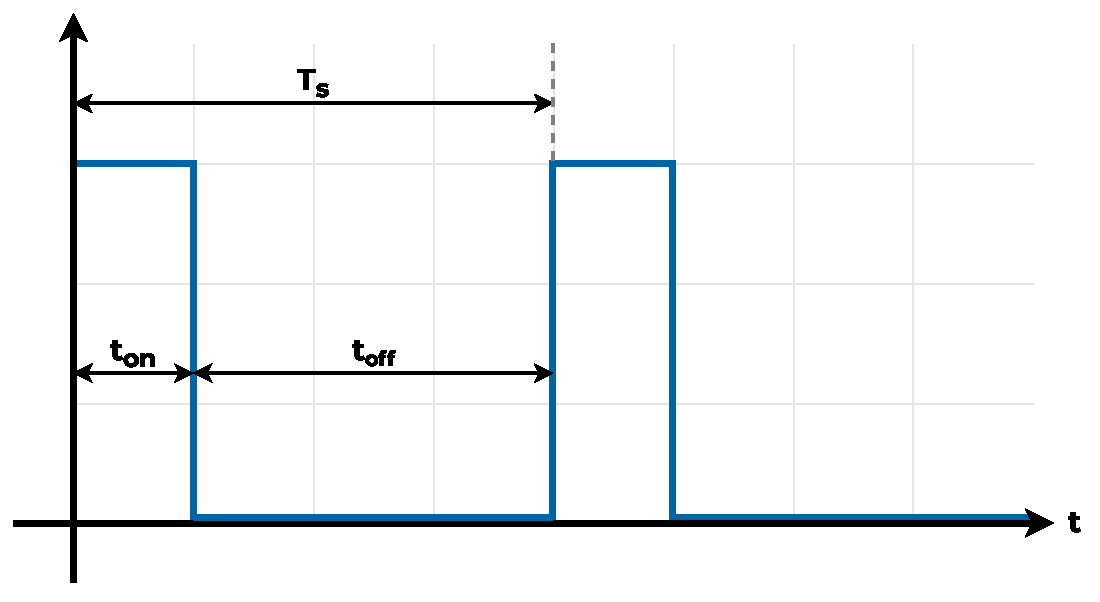
\includegraphics[scale=0.5]{Imagenes/Duty Cycle.pdf}
    \caption{Una forma de onda cuadrada con ciclo de trabajo $D$ del 25 \%.}
    \label{dutycycle}
\end{figure}

Los convertidores CC-CC conmutados se clasifican en dos grandes grupos, usando como criterio la existencia de aislación galvánica entre la entrada no regulada y la salida regulada:

\begin{itemize}
    \item {\SemiBold Convertidores No Aislados:} son los convertidores que no tienen aislación galvánica entre entrada y salida, como por ejemplo los convertidores reductores y elevadores (\textit{buck} y \textit{boost}), y por lo tanto son los mas simples de los dos tipos.
    \item {\SemiBold Convertidores Aislados:} son los convertidores que tienen su entrada y salida aisladas galvánicamente por medio de un transformador de alta frecuencia, por ejemplo los de tipo \textit{flyback} y \textit{forward}. El convertidor de esta plataforma, de tipo puente completo, cae dentro de esta categoría.
\end{itemize}

En la siguiente sección se va a detallar el funcionamiento del convertidor no aislado más sencillo, el convertidor reductor, a manera de introducir los principios de funcionamiento de convertidores conmutados que van a ser necesarios para luego poder entender las topologías más complejas que se utilizan en esta plataforma.\\

\subsubsection{El Convertidor Reductor}

La forma más básica posible de un convertidor conmutado tiene un esquema circuital similar al convertidor lineal mencionado más arriba, con la diferencia de que el transistor, (que previamente actuaba como una resistencia variable para conformar el divisor resistivo) en este caso, actúa como el interruptor del circuito, conmutando entre llave abierta y cerrada (figura \ref{proto_reductor}). Para este análisis vamos a considerar que el dispositivo semiconductor actúa como una llave ideal, sin impedancia cuando está cerrado y con impedancia infinita cuando está abierto.\\

\begin{figure}[h]
    \centering
    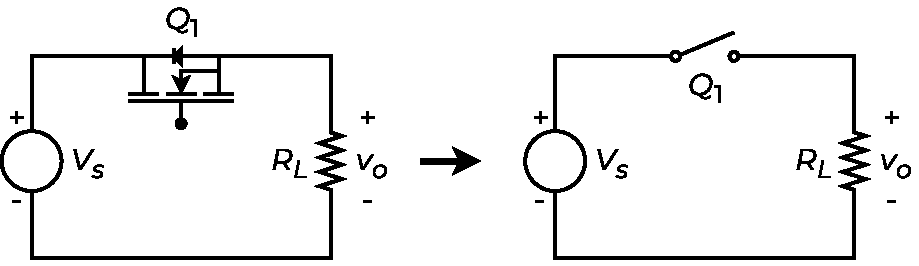
\includegraphics[scale=0.6]{Imagenes/Proto Reductor.pdf}
    \caption{Circuito de un convertidor conmutado básico, y su equivalente con el transistor $Q_1$ como llave ideal.}
    \label{proto_reductor}
\end{figure}

Entonces, si se aplica una señal de control como la de la figura \ref{dutycycle} al interruptor, durante un período $T_s$ de la señal ocurren dos cosas distintas:
"
\begin{itemize}
    \item {\SemiBold Durante el tiempo $\mathbf{t_{on}}$}, el transistor se comporta como una llave cerrada y permite la libre circulación de corriente. Entonces, esta corriente circula por la carga $R_L$, donde, por la Ley de Ohm, cae una tensión igual a la tensión de entrada, es decir, que la tensión de salida {\Medium \textit{v\textsubscript{o}} es igual a la tensión de entrada \textit{V\textsubscript{s}}}.
    \item {\SemiBold Durante el tiempo $\mathbf{t_{off}}$}, el transistor pasa a comportarse como una llave abierta, por lo que restringe completamente la circulación de corriente. Por lo tanto, la caída de tensión en la carga $R_L$ es nula, es decir, que la tensión de salida {\Medium \textit{v\textsubscript{o}} es nula}.
\end{itemize}

Uniendo estos dos comportamientos, se puede ver que la forma de la tensión de salida es análoga a la forma de onda cuadrada que controla al interruptor (de la figura \ref{dutycycle}), oscilando entre \SI{0}{\volt} y $V_s$.

\begin{equation}\label{valor_medio_reductor}
    \bar{v}_o = \frac{1}{T_s}\int\limits^{T_s}_0 v_0(t) dt = \frac{1}{T_s}\int\limits^{DT_s}_0 V_s dt = V_s\cdot D \leq V_s
\end{equation}

Calculando el valor medio de $v_o$ en la ecuación \ref{valor_medio_reductor}, este resulta ser directamente proporcional al ciclo de trabajo de la señal de control, variando entre \SI[]{0}[]{\volt} y la tensión de entrada $V_s$, para ciclos de trabajo entre \num{0} y \num{1} respectivamente. Es decir, la {\Medium tensión media de salida es menor o igual a la de entrada} (esto se puede ver sin necesidad de cálculo, ya que si la salida es igual a la entrada por una proporción del tiempo total, su valor medio necesariamente debe ser menor, o como mucho igual, al valor de la entrada) y se controla directamente con la variación de $D$.\\

En principio, si se considera el transistor como interruptor ideal, la eficiencia de este dispositivo es del 100 \%, ya que durante el tiempo $t_{off}$ no circula ninguna corriente (por lo tanto no hay disipación de ningún tipo), y durante $t_{on}$ no hay caída de tensión en el transistor. En la realidad, los transistores no actúan como llaves ideales, si no que tienen ciertas no idealidades que resultan en pérdidas de energía: no tienen impedancia perfectamente nula como llave cerrada, ni impedancia infinita como llave abierta, además de poseer pérdidas a la hora de conmutar.\\

Sin embargo, en muchos casos y aplicaciones (incluido el de este trabajo) no es suficiente obtener una salida de pulsos y controlar su tensión media, si no que se necesita obtener una tensión puramente continua directamente en la salida, como puede ser el caso para una fuente de alimentación.\\

Para solucionar este problema, se agrega un filtro pasa-bajos LC a la salida luego del interruptor, que se encarga de eliminar los componentes de alta frecuencia relacionados a la conmutación, dejando pasar únicamente los componentes de continua. El convertidor que resulta es la topología de convertidor CC-CC conmutado más sencilla: el {\Medium convertidor reductor} o {\Medium \textit{buck}} de la figura \ref{reductor}, que obtiene su nombre porque, como se ve en la ecuación \ref{valor_medio_reductor}, reduce la tensión de entrada.\\

\begin{figure}[h]
    \centering
    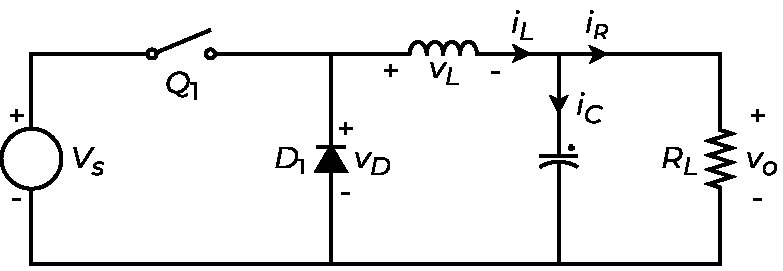
\includegraphics[scale=0.6]{Imagenes/Reductor.pdf}
    \caption{Circuito de un convertidor reductor o buck, con componentes ideales.}
    \label{reductor}
\end{figure}

Además del filtro ya mencionado, se agrega un diodo de rueda libre o \textit{flyback} en derivación entre el transistor y el inductor (diodo $D_1$ de la figura \ref{reductor}). Este dispositivo cumple la función de proveer un camino de circulación para la corriente $i_L$ del inductor cuando el interruptor se encuentra abierto, que resulta necesario ya que la corriente sobre un inductor no puede variar abruptamente. Entonces, cuando el interruptor está abierto, el diodo entra en polarización directa y permite la circulación de corriente; mientras que cuando está el interruptor cerrado, el diodo se polariza con una tensión inversa $V_s$ y actúa como un circuito abierto, eliminando su influencia sobre el convertidor durante $t_{on}$.\\

Durante su funcionamiento en estado estacionario, los convertidores reductores (y todos los convertidores CC-CC) tienen las siguientes propiedades:

\begin{itemize}
    \item La corriente $i_L$ sobre el inductor es periódica de período $T_s$, es decir, $i_L(t+T_s) = i_L(t)$.
    \item La tensión media $\bar{V}_L$ que cae en el inductor es nula, ya que si no lo fuera su corriente crecería sin límite.
    \item La corriente media $\bar{i}_C$ que circula por el capacitor es nula, ya que si no lo fuera su tensión crecería sin límite.
    \item La potencia absorbida por la carga es igual a la potencia entregada por la fuente. Para componentes no ideales, las pérdidas son entregadas por la fuente de entrada.
\end{itemize}

\paragraph{Análisis Detallado}

Ahora se va a realizar un análisis más en profundidad de la topología. Pero antes, es necesario aclarar el conjunto de condiciones que se asumirán, necesarias para simplificar y facilitar la comprensión de esta explicación:

\begin{enumerate}
    \item El circuito opera en estado estacionario, es decir que todos las respuestas transitorias ya se extinguieron.
    \item La corriente del inductor es continua, es decir que circula siempre en la misma dirección.
    \item El capacitor $C$ es lo suficientemente grande como para mantener la tensión de salida constante.
    \item El período de conmutación es $T_s$, con $t_{on} = DT_s$ y $t_{off} = (1-D)T_s$.
    \item Todos los componentes son ideales.
\end{enumerate}

Para poder determinar la tensión de salida $v_o$ del sistema, se va a determinar primero la corriente y tensión del inductor $L$ del filtro de salida, para cada uno de los dos estados del circuito: {\Medium llave abierta} y {\Medium llave cerrada}. Para cumplir la condición de funcionamiento en estado estacionario, la corriente $i_L$ debe tener una variación total nula durante un período $T_s$ (es decir que la corriente debe ser la misma al principio y final de un ciclo), y, como se mencionó más arriba, su tensión media debe ser idénticamente nula.\\

\subparagraph{Llave Cerrada}

Al estar la llave cerrada durante el tiempo $t_{on} = DT_s$, la tensión de entrada $V_s$ cae directamente sobre el diodo $D_1$, polarizándolo con una tensión inversa que no permite que circule corriente por el mismo, y en consecuencia, neutralizando su efecto sobre el circuito. Se puede ver el circuito equivalente para este estado en la figura \ref{reductor_llave_cerrada}.\\

\begin{figure}[h]
    \centering
    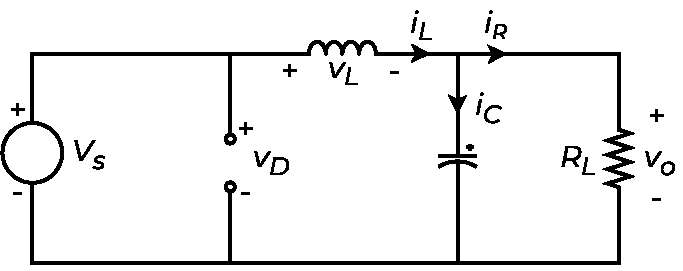
\includegraphics[scale=0.6]{Imagenes/Reductor Llave Cerrada.pdf}
    \caption{Circuito equivalente de un convertidor reductor para llave cerrada.}
    \label{reductor_llave_cerrada}
\end{figure}

Entonces, recordando que la tensión que cae sobre una bobina es proporcional a la corriente que circula sobre ella (con $L$ como constante de proporcionalidad), la tensión sobre el inductor del circuito resulta

\begin{equation}\label{ec_tensionL_cerrada}
    v_L = V_s - v_o = L\frac{di_L}{dt}
\end{equation}

Como la tensión, y por lo tanto la derivada de la corriente, son valores constantes y positivos, la corriente por el inductor es descrita por una recta de pendiente positiva. El cambio neto de corriente $(\Delta i_L)_{cerrado}$ mientras la llave permanece cerrada es entonces

\begin{equation*}
    \frac{di_L}{dt} = \frac{(\Delta i_L)_{cerrado}}{\Delta t} = \frac{(\Delta i_L)_{cerrado}}{DT_s} = \frac{V_s - v_o}{L}\\
\end{equation*}

Reorganizando:

\begin{equation}\label{deltaiL_cerrada}
    \boxed{
        (\Delta i_L)_{cerrado} = \left(\frac{V_s - v_o}{L}\right)DT_s
    }
\end{equation}

\subparagraph{Llave abierta}

Ahora, al abrirse la llave durante el tiempo $t_{off} = (1-D)T_s$, el diodo entra en modo de polarización directa, permitiendo la circulación de la corriente acumulada en el inductor. La fuente queda desconectada y no entrega energía, conformándose el circuito equivalente de la figura \ref{reductor_llave_abierta}.\\

\begin{figure}[h]
    \centering
    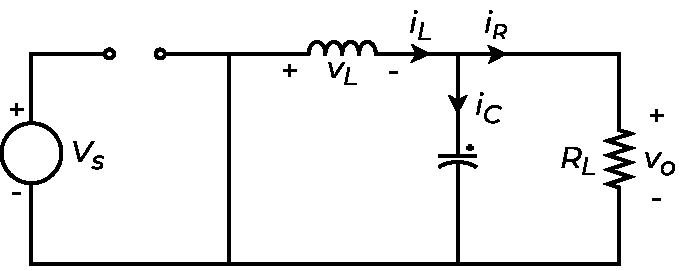
\includegraphics[scale=0.6]{Imagenes/Reductor Llave Abierta.pdf}
    \caption{Circuito equivalente de un convertidor reductor para llave abierta.}
    \label{reductor_llave_abierta}
\end{figure}

En este intervalo de tiempo, la tensión sobre el inductor es

\begin{equation}\label{ec_tensionL_abierta}
    v_L = -v_o = L\frac{di_L}{dt}
\end{equation}

Entonces, aplicando un razonamiento análogo al del período de llave cerrada, con la diferencia que en este caso, al ser la tensión $v_L$ negativa, la recta de la corriente $i_L$ es decreciente, se obtiene que el cambio neto de corriente $(\Delta i_L)_{abierto}$ mientras la llave está abierta es

\begin{equation*}
    \frac{di_L}{dt} = \frac{(\Delta i_L)_{abierto}}{(1-D)T_s} = \frac{-v_o}{L}\\
\end{equation*}

Reordenando:

\begin{equation}\label{deltaiL_abierta}
    \boxed{
        (\Delta i_L)_{abierto} = -\left(\frac{v_o}{L}\right)(1-D)T_s
    }
\end{equation}

Como se mencionó antes, para este análisis se asumió el funcionamiento en estado estacionario, por lo que la suma de los cambios netos de corriente de las ecuaciones \ref{deltaiL_cerrada} y \ref{deltaiL_abierta} para ambos estados del circuito debe ser igual a cero.

\begin{equation}
    (\Delta i_L)_{cerrado} + (\Delta i_L)_{abierto} = 0
\end{equation}

Reemplazando ambas variables por sus expresiones, se obtiene

\begin{equation*}
    \left(\frac{V_s - v_o}{L}\right)DT_s - \left(\frac{v_o}{L}\right)(1-D)T_s  = 0
\end{equation*}

Despejando de la ecuación anterior, se consigue una expresión para la tensión de salida $v_o$ de este convertidor.

\begin{equation}\label{vo_reductor}
    \boxed{
        v_o = V_sD
    }
\end{equation}

Este resultado es idéntico al de la ecuación \ref{valor_medio_reductor} obtenido para el convertidor básico de la figura \ref{proto_reductor}. En conclusión, {\Medium en un convertidor reductor, la tensión de salida siempre es menor o igual a la entrada}.\\

Evidentemente, por el resultado obtenido en la ecuación \ref{vo_reductor}, la salida se controla únicamente con el ciclo de trabajo $D$ del transistor. Por ejemplo, si aumenta la tensión de alimentación $V_s$ pero se desea mantener $v_o$ a un nivel constante, se compensa este aumento con una disminución del ciclo de trabajo (o viceversa). Si se agrega un sensor que mida la tensión de salida, se puede implementar un lazo de control automático que mantiente $v_o$ fijada a una referencia mediante la variación de $D$.\\

\subsubsection{Convertidores CC-CC Aislados}

Habiendo entendido el funcionamiento del convertidor reductor en la anterior sección (que cae en la categoría de convertidores CC-CC no aislados), ahora vamos a pasar a los convertidores CC-CC aislados, categoría en la cual se encuentra el convertidor tipo puente completo de esta plataforma.\\

Los convertidores aislados son generalmente utilizados en fuentes de alimentación de corriente continua, y a diferencia de los no aislados, tienen un transformador de alta frecuencia de por medio, para generar una {\Medium aislación galvánica entre la entrada y la salida}. Además, como los transformadores solo conducen corriente alterna, a su salida debe incluirse algún tipo de circuito rectificador para transformarla a corriente continua para alimentar a la carga.\\

Es claro que el adicionado de un transformador agrega una mayor complejidad al circuito. Entonces, ¿por qué se busca esta aislación galvánica? Sin la aislación interpuesta, nuestra salida va a compartir la conexión a tierra con la fuente de alimentación, (que suelen tener tierras muy ruidosas) introduciendo ruido no deseado a la salida. En muchas aplicaciones hay una gran sensibilidad al ruido en la carga, por lo que es deseable mantenerlo lo más bajo posible, incluso si agrega complejidad al diseño. Adicionalmente, la presencia de aislación galvánica presenta una ventaja en cuestiones de seguridad, tanto para proteger a quienes operan con el circuito como para protección de los componentes del mismo circuito.\\

Otra ventaja es la mayor flexibilidad que un transformador en la etapa de continua aporta al diseño, ya que variando la relación de vueltas entre bobinados (por ejemplo con el uso de múltiples bobinados) se puede variar la tensión de salida entre distintos niveles.\\

Ahora se procederá a derivar las distintas topologías de convertidores aislados, partiendo del convertidor reductor (no aislado) que se explico más arriba. Estos convertidores que obtendremos los vamos a llamar {\Medium convertidores aislados derivados del reductor} o \textit{isolated buck-derived converters}\textsuperscript{\cite{SoftSwitchPWM}}, comenzando por el convertidor \textit{forward}.\\

\paragraph{El Convertidor Forward}

Si tomamos el circuito del reductor de la figura \ref{reductor}, y le agregamos un transformador de alta frecuencia entre la llave $Q_1$ y el diodo $D_1$, se obtiene la aislación galvánica buscada, como se observa en el circuito de la figura \ref{desarrollo_forward}.\\

\begin{figure}[h]
    \centering
    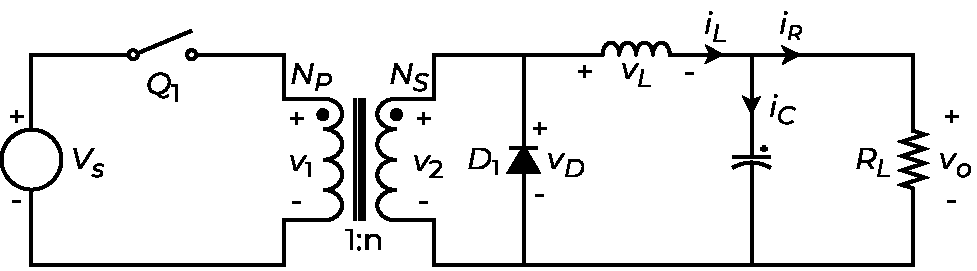
\includegraphics[scale=0.6]{Imagenes/Desarrollo Forward 1.pdf}
    \caption{Convertidor reductor con un transformador interpuesto entre la llave $Q_1$ y el diodo $D_1$.}
    \label{desarrollo_forward}
\end{figure}

Cuando la llave está cerrada, la tensión $V_s$ de entrada se aplica sobre el bobinado primario del transformador, traduciéndose a una tensión de la misma polaridad (por la ubicación de los puntos homólogos) pero afectada por la relación de vueltas $n$. Esto genera que el núcleo ferromagnético del transformador se magnetice, y aumente su flujo de magentización $\phi_m$.\\

Cuando la llave se abre, la corriente del inductor de filtro circula por el diodo $D_1$, cortocircuitando el bobinado secundario del transformador. Esto fuerza que la tensión y la corriente del transformador se anulen, y por lo tanto, el flujo magnetizante se mantiene constante.\\

Entonces, durante un período de conmutación $T_s$, el flujo $\phi_m$ del núcleo del transformador tiene un incremento neto. Pasados suficientes períodos, este flujo aumenta lo suficiente como para saturar el transformador, cosa que no es deseable, ya que puede resultar en corrientes elevadas y eventualmente, la destrucción del transistor de potencia que actúa como llave.\\

Para solucionar este problema, se debe agregar algún circuito auxiliar de restablecimiento del núcleo que, durante el período en el que la llave está abierta, aplique una tensión negativa en el bobinado primario y permita una circulación inversa de corriente para restablecer el flujo magnetizante a su valor original.\\

Pero, al aplicar esta tensión negativa en el primario, se refleja en una tensión negativa del secundario que polariza en directa a $D_1$, cortocircuitando este bobinado. Para arreglar este inconveniente, se puede agregar un diodo rectificador $D_R$ en serie con el bobinado secundario, que no permita la circulación inversa de corriente.\\

Teniendo esto en cuenta, se ve en la figura \ref{forward} el circuito de un {\Medium convertidor \textit{forward}} derivado de un reductor, dónde se agregaron el circuito de restablecimiento de núcleo, compuesto por un bobinado auxiliar y un diodo $D_r$ en serie; en paralelo con el bobinado primario y la llave $Q_1$ (en posiciones invertidas); y el diodo rectificador $D_R$ en el secundario (respecto a la figura \ref{desarrollo_forward}).\\

\begin{figure}[h]
    \centering
    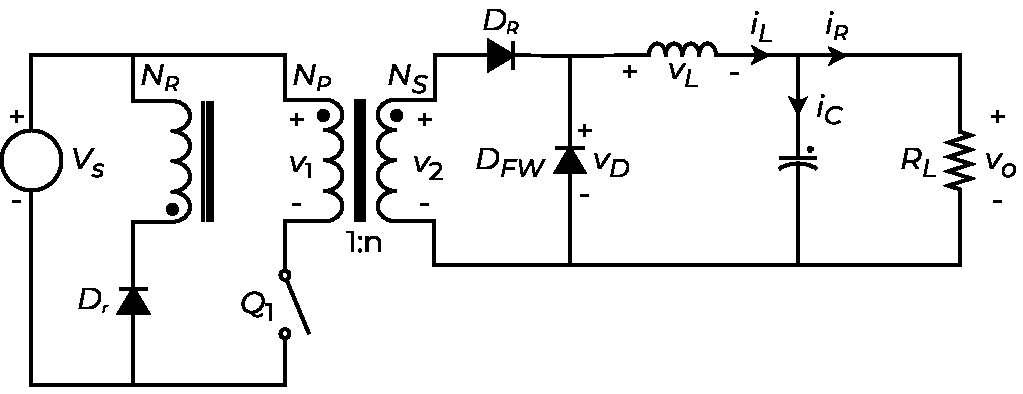
\includegraphics[scale=0.6]{Imagenes/Forward.pdf}
    \caption{Circuito de un convertidor aislado tipo forward, desarrollado a partir del circuito de un reductor.}
    \label{forward}
\end{figure}

Dado que este circuito es similar a un convertidor reductor, solo que con un transformador de relación de vueltas $n$ interpuesto (y los circuitos auxiliares que no afectan la salida), se puede ver que su relación entrada-salida será similar a la del convertidor en el que se basa (ecuación \ref{vo_reductor}) pero afectada por la relación de vueltas del transformador.\textsuperscript{\cite{PotenciaHart}}

\begin{equation}\label{vo_forward}
    \boxed{
        v_o = \left(\frac{N_S}{N_P}\right)V_sD = nV_sD
    }
\end{equation}

Con estos resultados se puede ver la flexibilidad aportada por el transformador: a pesar de ser muy similar a un circuito que solo permite reducir la tensión, con la relación de vueltas se puede obtener cualquier nivel de tensión que se desee a la salida. Sin embargo, al tener que restablecer la magnetización del núcleo, se suele limitar el ciclo de trabajo a 50 \% para poder lograr la demagnetización completa.\\

Además, con el circuito de restablecimiento de flujo, el estrés de tensión sobre la única llave del circuito se duplica respecto al convertidor reductor: al estar la llave abierta, debe soportar una tensión de dos veces la tensión de entrada $V_s$ (para bobinados $N_P$ y $N_R$ iguales). Esto puede ser problemático para aplicaciones de alta tensión, ya que los transistores de alta tensión que se requieren son mas caros y suelen tener desempeño degradado a altas frecuencias de conmutación.\\

\subparagraph{Forward de Doble Llave}

Para solucionar este inconveniente, se puede diseñar un converitdor forward de dos llaves o \textit{double-ended}, que disminuye el estrés de tensión de cada llave a $V_s$ sin cambiar la tensión de salida, que se mantiene igual a la ecuación \ref{vo_forward} del convertidor forward común.\\

Entonces, si agregamos una segunda llave $Q_2$ en serie a la llave original, ambas conmutando al mismo tiempo, la tensión de llave abierta se reparte entre ambas llaves, logrando lo que se buscaba. Para asegurar que en cada llave caiga la tensión $V_s$ correspondiente, se agregan los diodos $D_1$ y $D_2$, conectados entre el terminal negativo del transformador y $V_s$, y entre el terminal negativo de $V_s$ y el terminal positivo del transformador respectivamente.\\

Estos diodos, durante el tiempo en que ninguna llave conduce, permiten el flujo inverso de corriente por el bobinado, cumpliendo el rol adicional de circuito de restablecimiento de $\phi_m$. Esto hace redundante al bobinado $N_R$ y su diodo $D_r$, por lo que se pueden remover, resultando en el circuito de la figura \ref{forward_doubleended}.\\

\begin{figure}[h]
    \centering
    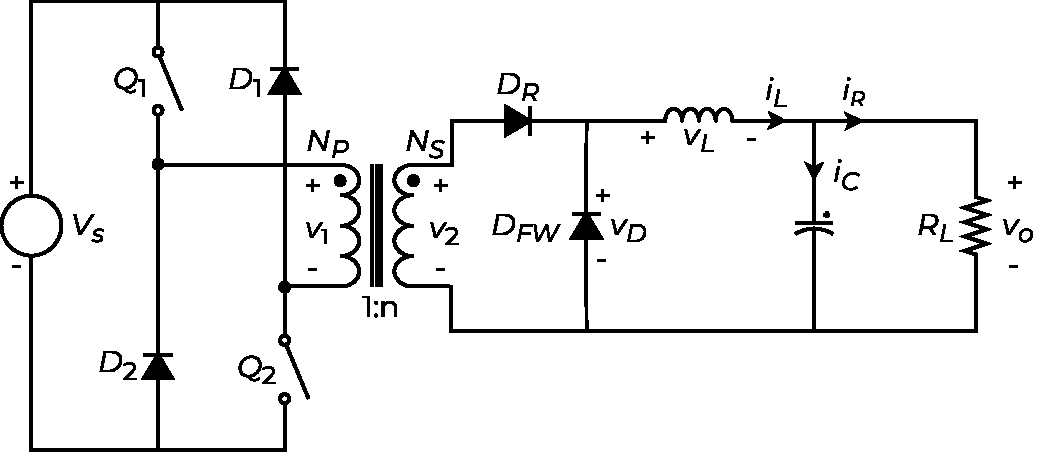
\includegraphics[scale=0.6]{Imagenes/Forward Double-Ended.pdf}
    \caption{Circuito de un convertidor aislado tipo forward de doble llave o double-ended.}
    \label{forward_doubleended}
\end{figure}

Una consecuencia que existe para ambos tipos de convertidores forward (normal y double-ended), es que al estar el ciclo de trabajo limitado a la mitad del período, los requerimientos de filtrado aumentan considerablemente. Esto requiere de la utilización de una bobina de mucha mayor inductancia, aumentando su costo y tamaño, además de introducir una gran cantidad de armónicos de la frecuencia de conmutación.\textsuperscript{\cite{SoftSwitchPWM}}\\

Entonces, se debe encontrar un circuito que sea capaz de obtener una tensión rectificada de secundario que supere el 50 \% de ciclo de trabajo, disminuyendo los requerimientos del filtro y la presencia de armónicos no deseados. Vamos a obtener este circuito partiendo del circuito del convertidor forward de una llave de la figura \ref{forward}.\\

\paragraph{El Convertidor Push-Pull}

Una posible solución podría ser la conexión de dos convertidores forward en paralelo en el primario, que luego compartan el diodo $D_1$ y el filtro de salida LC del lado secundario. Los interruptores $Q_1$ y $Q_2$ deben operar de manera complementaria, con $Q_1$ conduciendo cuando $Q_2$ se abre y viceversa (ambos con el mismo ciclo de trabajo); obteniendo una tensión rectificada del doble de ciclo de trabajo de cada llave.\\

\begin{figure}[h]
    \centering
    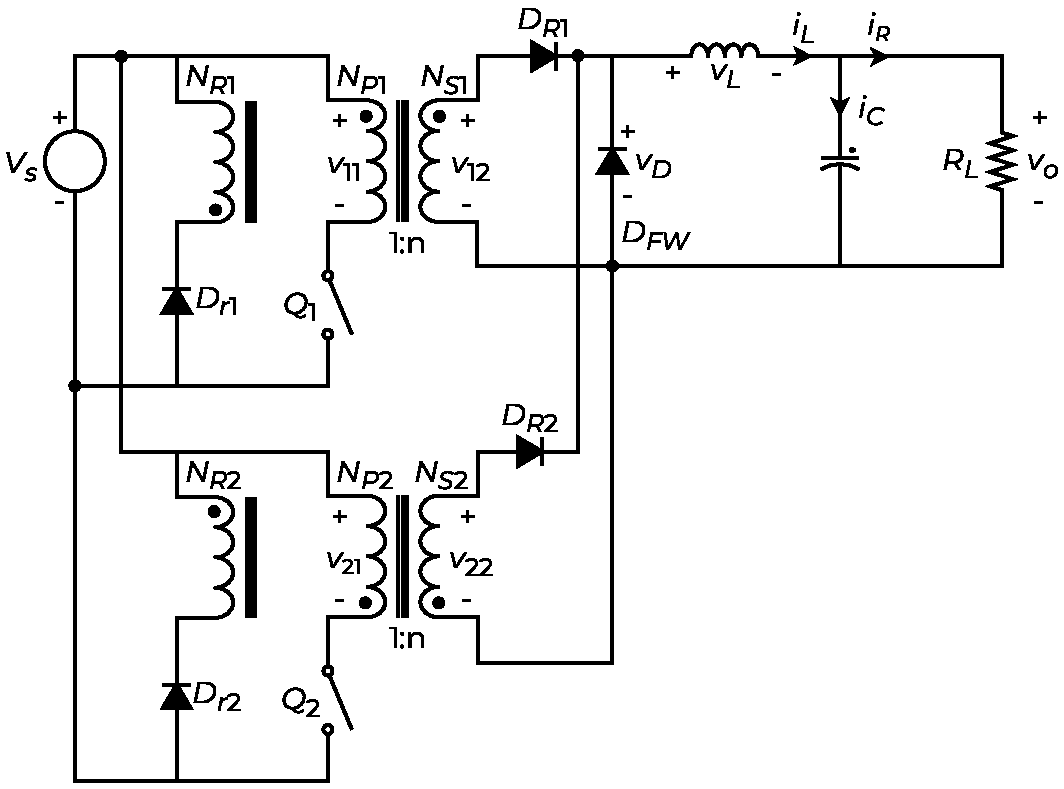
\includegraphics[scale=0.6]{Imagenes/Desarrollo Push-Pull 1.pdf}
    \caption{Dos convertidores forward conectados en paralelo en el primario, compartiendo diodo y filtro de salida.}
    \label{desarrollo_pushpull}
\end{figure}

El circuito resultante de la figura \ref{desarrollo_pushpull}, sin embargo, se puede simplificar. Si hacemos que ambos bobinados primarios compartan su núcleo magnético; entonces, se puede agregar un diodo en antiparalelo a cada llave, de manera que cada uno de estos diodos, junto con los bobinados que tienen en serie, pueden funcionar como circuitos de restablecimiento del núcleo cuando la otra llave esta conduciendo (es decir, cuando $Q_2$ conduce, el diodo antiparalelo de $Q_1$ y su bobinado restablecen la magentización del núcleo, y viceversa).\\

Entonces, los circuitos de restablecimiento heredados del convertidor forward son redundantes, y por lo tanto se pueden remover para simplificar el circuito, resultando en el {\Medium convertidor \textit{push-pull}} que se observa en la figura \ref{pushpull}. Además, el diodo de rueda libre $D_{FW}$ se puede remover, ya que con el rectificador de punto medio conformado por $D_{R1}$ y $D_{R2}$ se forma un camino para la circulación de la corriente del inductor.\\

\begin{figure}[h]
    \centering
    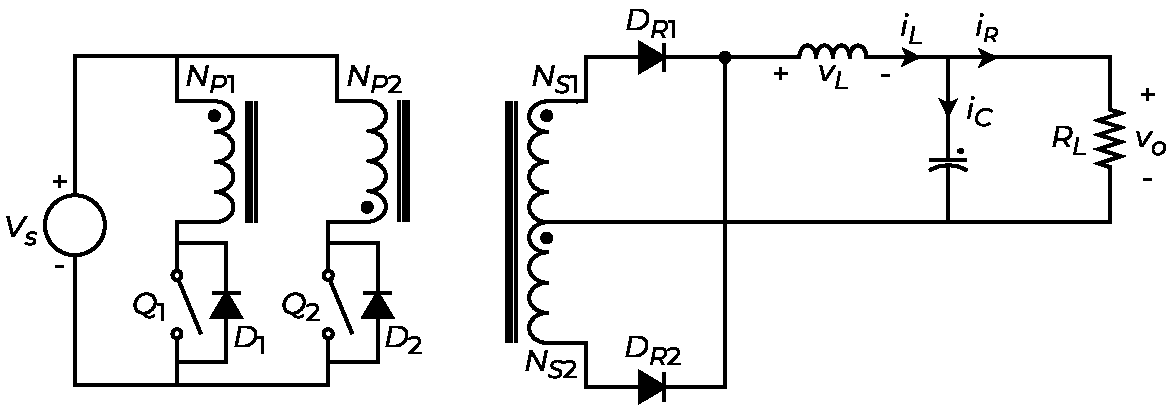
\includegraphics[scale=0.6]{Imagenes/Push-Pull.pdf}
    \caption{Circuito de un convertidor aislado tipo push-pull.}
    \label{pushpull}
\end{figure}

Para obtener su tensión de salida no es necesario realizar toda la deducción matemática. Al ser esta topología esencialmente dos convertidores forward que conducen de manera alternada (cada columna del primario es equivalente a un covertidor forward), el ciclo de trabajo de la onda rectificada es el doble del de cada una de las columnas. Entonces, es razonable decir que su tensión $v_o$ es dos veces la del convertidor forward (ecuación \ref{vo_forward})\textsuperscript{\cite{PotenciaHart}}, siempre que ambos bobinados primarios y secundarios sean iguales.

\begin{equation}\label{vo_pushpull}
    \boxed{
        v_o = 2\left(\frac{N_{S1}}{N_{P1}}\right)V_sD = 2\left(\frac{N_{S2}}{N_{P2}}\right)V_sD
    }
\end{equation}

Esta topología soluciona los problemas de rectificación que tienen los convertidores forward, pero cada llave debe soportar $2V_s$ de tensión cuando está abierta (porque son dos forward intercalados), introduciendo de vuelta la problemática que se solucionó con el forward double-ended. Sería desable entonces, encontrar una topología aislada que sea capaz de solucionar ambos inconvenientes.\\

\subsubsection{El Convertidor de Puente Completo}

Este tipo particular de convertidor aislado, que es el elegido para esta plataforma, es el más complejo dentro de su categoría: utiliza cuatro llaves distintas, y por lo tanto tiene un sobresaliente rendimiento para aplicaciones de alta potencia y tensión. Se va a obtener su circuito a partir de las topologías previamente explicadas, detallando sus ventajas y desventajas. Luego se va a desarrollar un modelo matemático para representarlo y se explicará la forma de controlarlo mediante el método \textit{phase-shift}.\\

Si tomamos el circuito del convertidor forward de dos llaves de la figura \ref{forward_doubleended}, se puede concebir una conxión alternativa para el mismo, donde intercambiamos los lugares de la llave y el diodo en cada una de las dos columnas, e invertimos la posición del punto homólogo del secundario. Entonces, cuando ambas llaves están cerradas (recordando que en esta topología ambas llaves conmutan en conjunto) el núcleo se magnetiza negativamente, y una vez que se abren, lo corriente (positiva) que circula por los diodos restablece los niveles de magnetización.\\

\begin{figure}[h]
    \centering
    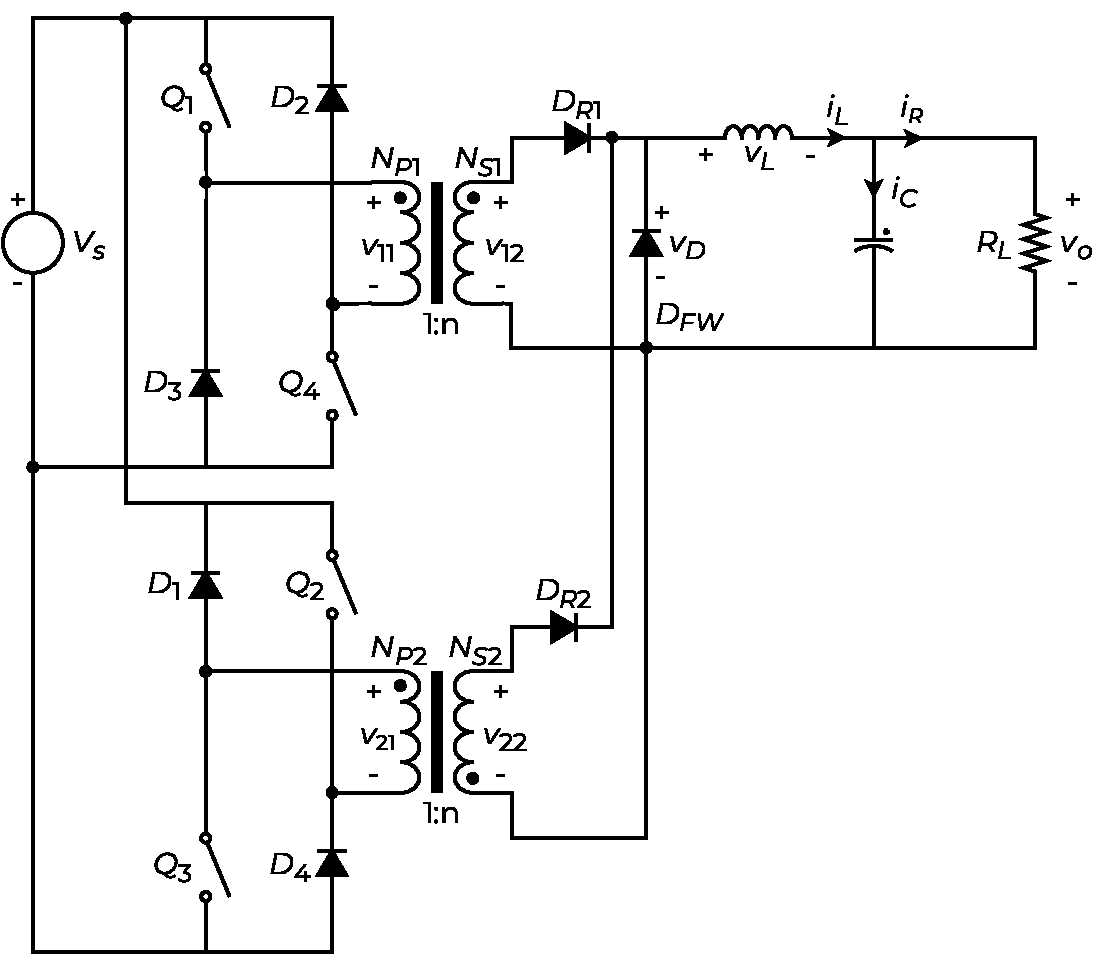
\includegraphics[scale=0.6]{Imagenes/Desarrollo Full-Bridge.pdf}
    \caption{Dos variantes de convertidores forward de dos llaves conectados en paralelo.}
    \label{desarrollo_fullbridge}
\end{figure}

Si conectamos ambas variantes del forward de dos llaves en paralelo, obtenemos el circuito de la figura \ref{desarrollo_fullbridge}, donde las llaves $Q_1$ y $Q_4$ conmutan en sincronía, y desfasadas un tiempo $T_s/2$ de $Q_2$ y $Q_3$ (que también conmutan en sincronía).\\

Siguiendo los pasos de la derivación del push-pull, si hacemos que ambos bobinados primarios compartan un solo núcleo magnético y conectamos diodos antiparalelos a cada una de las llaves, el flujo magnetizante del núcleo puede ser restablecido por los diodos de $Q_1$ y $Q_4$ y el bobinado primario $N_{P1}$, o bien por los diodos de $Q_2$ y $Q_3$ y el bobinado primario $N_{P2}$.\\

Entonces, los diodos $D_1$ a $D_4$ provenientes de los convertidores forward resultan redundantes por la utilización de los diodos antiparalelos, y pueden ser removidos del circuito. Lo que queda entonces, es notar que ahora ambos bobinados primarios tienen formas de onda de tensión y corriente idénticas, por lo que pueden unirse sus terminales positivos y sus terminales negativos, quedando, efectivamente conectados en paralelo. Si ambos bobinados están conectados en paralelo, uno de ellos es redundante y se puede remover sin consecuencias para el funcionamiento del circuito.\\

Si aplicamos todos estos cambios al circuito de la figura \ref{desarrollo_fullbridge}, obtenemos el circuito de un {\Medium convertidor aislado de puente completo} o {\Medium \textit{full-bridge}} en la figura \ref{fullbridge_partido}. Al igual que en el desarrollo del push-pull, el diodo $D_{FW}$ también se puede eliminar ya que los diodos del rectificador de punto medio ya proveen un camino para la corriente del transistor.\\

\begin{figure}[H]
    \centering
    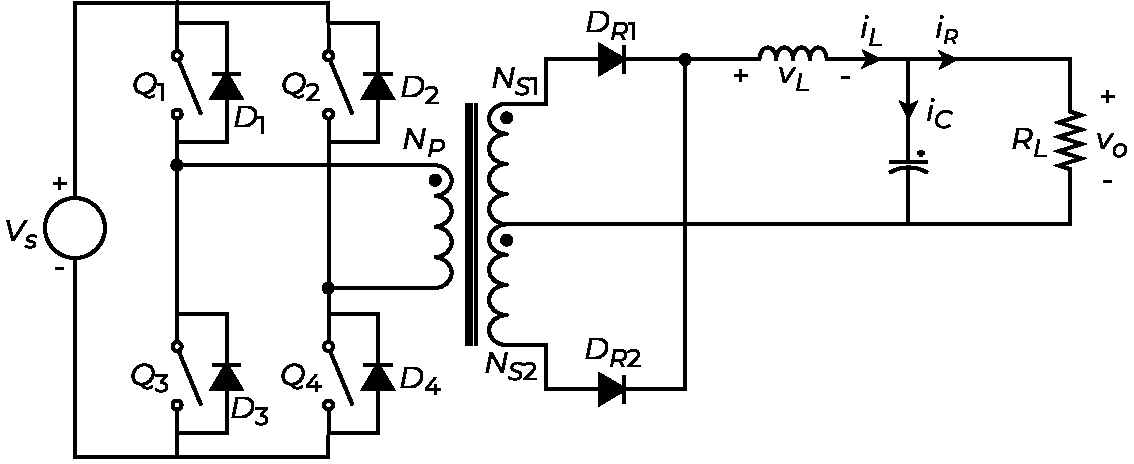
\includegraphics[scale=0.6]{Imagenes/Full Bridge Onda Completa.pdf}
    \caption{Circuito de un convertidor aislado tipo puente completo o full-bridge, con un rectificador de onda completa en el secundario.}
    \label{fullbridge_partido}
\end{figure}

Sin embargo, esta no es la topología exacta que se utiliza en este trabajo. Para simplificar la construcción del transformador de alta frecuencia y disminuir los requerimientos de desempeño impuestos a los diodos rectificadores del secundario, se utiliza un {\Medium rectificador de tipo puente completo} en el secundario como en la figura \ref{fullbridge}. Esta topología utiliza cuatro diodos en vez de dos, pero cada diodo debe soportar la mitad de la tensión inversa. Además, el transformador resulta más sencillo ya que solo tiene un bobinado secundario y no requiere tener punto medio.\\

\begin{figure}[h]
    \centering
    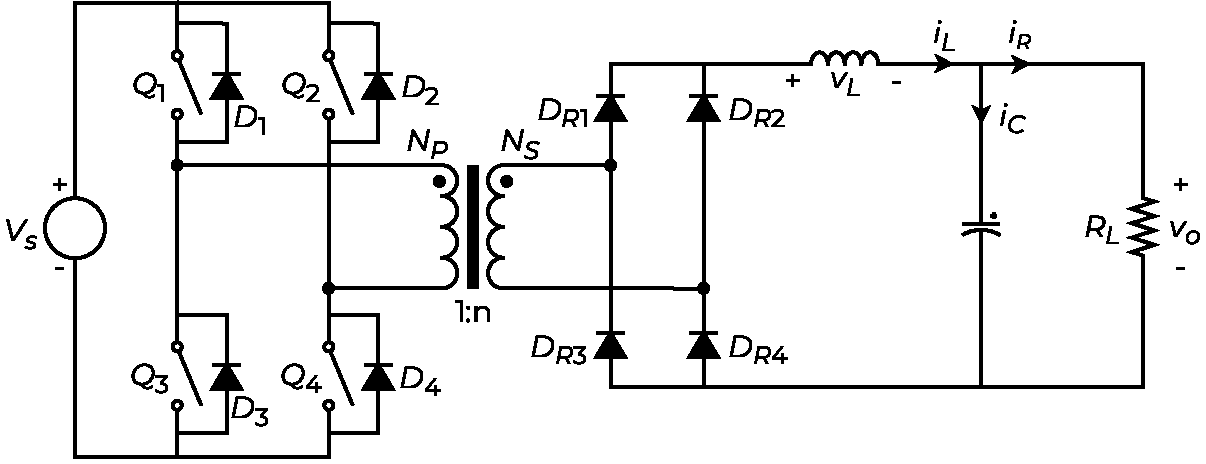
\includegraphics[scale=0.6]{Imagenes/Full Bridge.pdf}
    \caption{Circuito de un convertidor aislado tipo puente completo o full-bridge, con un rectificador de puente completo en el secundario.}
    \label{fullbridge}
\end{figure}

{\Large\Bold\scshape Sección por terminar.}\\
